% use paper, or submit
% use 11 pt (preferred), 12 pt, or 10 pt only

\documentclass[letterpaper, preprint, paper,11pt]{AAS}	% for preprint proceedings
%\documentclass[letterpaper, paper,11pt]{AAS}		% for final proceedings (20-page limit)
%\documentclass[letterpaper, paper,12pt]{AAS}		% for final proceedings (20-page limit)
%\documentclass[letterpaper, paper,10pt]{AAS}		% for final proceedings (20-page limit)
%\documentclass[letterpaper, submit]{AAS}			% to submit to JAS

\usepackage{overcite} % superscript reference numbers when cited
\usepackage{footnpag}			      	% make footnote symbols restart on each page
\usepackage{AAS_packages}

%\PaperNumber{XX-XXX}

\begin{document}

\title{Low-Thrust trajectory design near asteroids using invariant manifolds and reachability sets}

\author{Shankar Kulumani\thanks{Graduate Student, Mechanical and Aerospace Engineering, George Washington University, 801 22\textsuperscript{nd} St NW, Washington, DC 20052.}, and  
Taeyoung Lee\thanks{Associate Professor, Mechanical and Aerospace Engineering, George Washington University, 801 22\textsuperscript{nd} St NW, Washington, DC 20052.}
}


\maketitle{} 		


\section{Introduction}

% Introduction to why asteroid missions are important
Small bodies, such as asteroids and comets, are popular targets for spacecraft exploration missions.
Several recent missions, such as NASA's NEAR and JAXA Hyabusa, have returned new scientific insight into the solar system. 
These small bodies are remnants from the early period of the solar system and offer insight into the formation of the planets.
In addition, many small bodies are close to the Earth and can be explored with much lower energy requirements than other celestial bodies.
This lower cost makes them attractive targets for future manned missions, resource mining, and scientific missions.
Finally, near-Earth objects may pose a significant risk of collision and the development of impact mitigation technologies is an active area of research.
 
% Similarities with three body problem
% structure of dynamics is similar to the three body problem
% eq points and invariant manifolds exists
% much of the theory developed in three body system could be applied
The restricted full-two body problem describes the motion of a massless spacecraft under the influence of a rotating small body.
Typically, the dynamics are formulated in a rotating reference frame fixed to the surface of the body.
If we assume a uniformly rotating body, then the feasible motion of a spacecraft is constrained by a constant of motion, or Jacobi integral~\cite{scheeres1994,scheeres2012}.
This model is very similar to the well-known restricted three-body problem and much of the developed theory is also applicable to this problem~\cite{koon2011,ross2006}.
As in the three-body problem, relative equilibria exist as well as periodic orbits about them.
It has been shown that there exist multi-dimensional tubes, or invariant manifolds, of constant energy trajectories that span the state space. 
Associated with periodic solutions, these invariant manifolds allow for the spacecraft to traverse vast expanses of the state space with zero energy change. 
However, there has been much less investigation into the use of invariant manifolds near small bodies than in the three-body problem~\cite{herrera2014,mondelo2010}.
Utilizing the theory developed in the three-body problem allows for a new class of potential operations about small bodies.

% Challenges with previous approach
% herrera-sucarrat investigate invariant manifolds which pass near surface
% ellipsoid shape model and 2nd order gravity only
% propulsion system not considered
Reference~\citenum{herrera2014} investigated the invariant manifolds associated with periodic orbits about uniformly rotating non-spherical asteroids.
The invariant manifolds are computed for a variety of potential asteroid shape and spin rates with a focus on those which approach the surface. 
Potential landing trajectories are determined by utilizing portions of the invariant manifold which intersect the surface. 
In this manner, it may be possible to transition from orbit to landing with little to no propulsion costs. 
However, the analysis is based on a triaxial ellipsoid shape model and a second order and degree gravity model.
Many small bodies have strongly distended body shapes and the triaxial ellipsoid model is not a good approximation.
\begin{figure} 
	\centering 
	\begin{subfigure}[htbp]{0.5\textwidth} 
		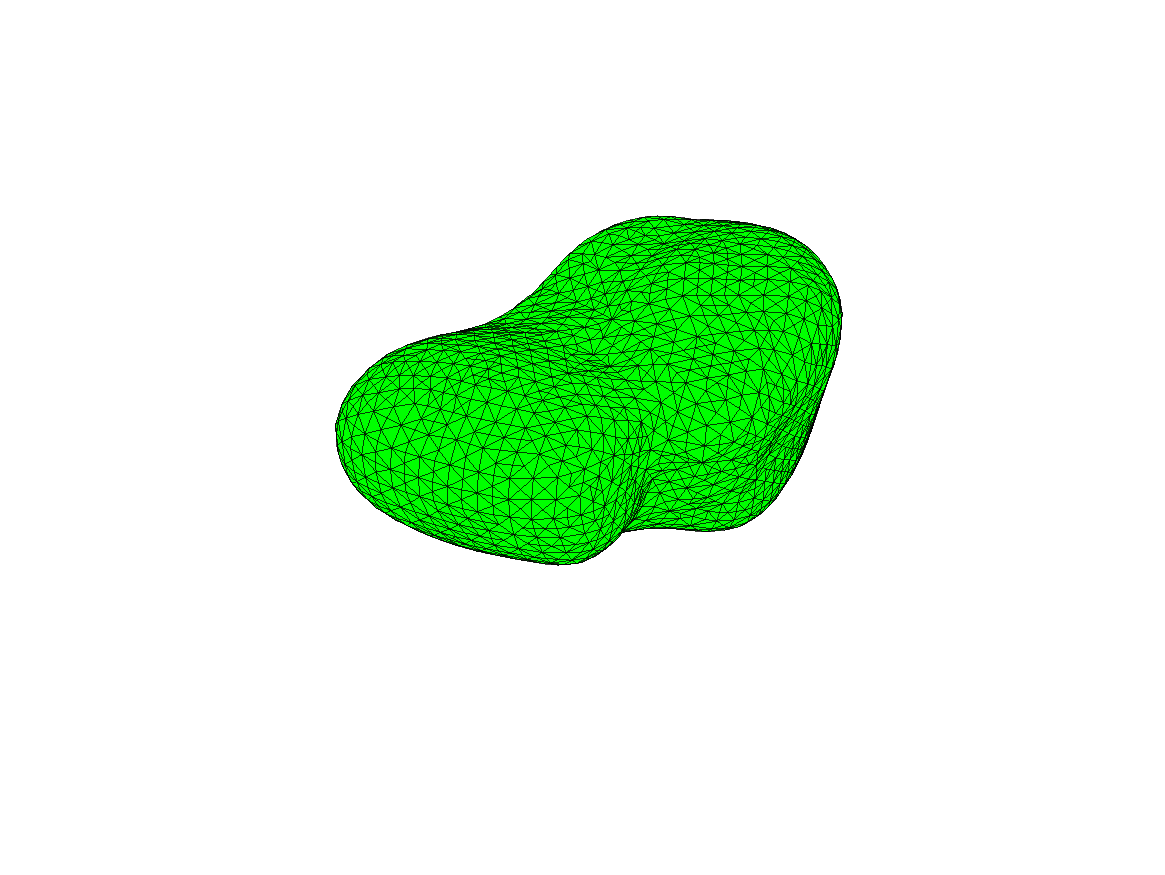
\includegraphics[width=\textwidth]{4769_castalia} 
		\caption{4769 Castalia} \label{fig:castalia} 
	\end{subfigure}~ %add desired spacing between images, e. g. ~, \quad, \qquad, \hfill etc. %(or a blank line to force the subfigure onto a new line) 
	\begin{subfigure}[htbp]{0.5\textwidth} 
		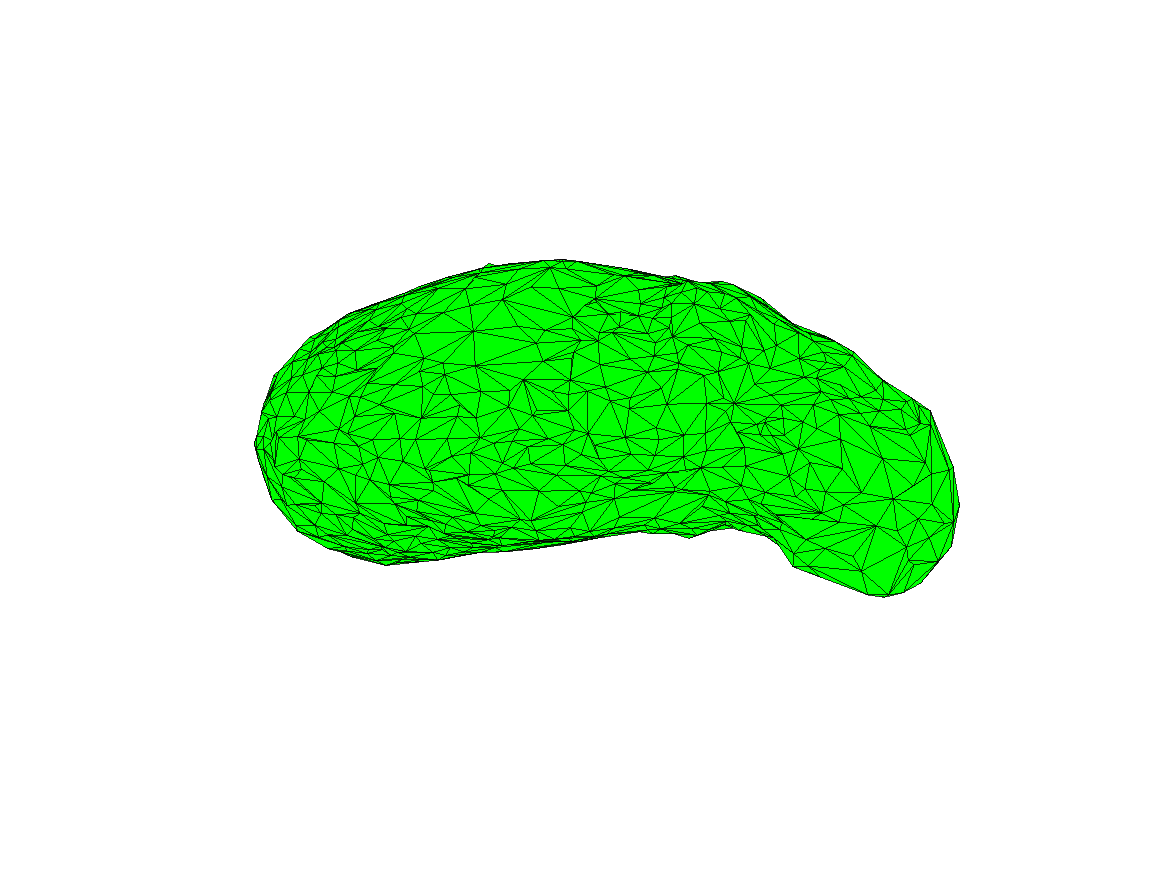
\includegraphics[width=\textwidth]{itokawa} 
		\caption{Itokawa} \label{fig:itokawa} 
	\end{subfigure} 
	\caption{Distended shape of asteroids 4769 Castalia and Itokawa}
	\label{fig:asteroid_shape} 
\end{figure}
In addition, a second degree and order spherical harmonic gravitational potential does not capture the higher order effects of the asteroid shape, especially when close to the surface of the body.

% mondelo looked at invariant manifolds to allow passage across resonance orbits
%spherical harmonic gravity model and shape based as triaxial ellipsoid (vesta is good model but smaller bodies have distended shapes)
% thrust not considered but rather only free trajectories
Reference~\citenum{mondelo2010} investigated the use of invariant manifolds for transfers around the asteroid Vesta.
The invariant manifolds are utilized to determine transfer trajectories across the 1:1 resonance orbit regime.
This analysis also utilized a truncated spherical harmonic representation of the gravitational potential. 
While well suited for Vesta, this type of model is less applicable for many distended bodies.
In addition, only control-free trajectories were investigated.
The spacecraft is limited to motion along the invariant manifold at a specific Jacobi constant value.
The equilibrium points and invariant manifolds are highly dependent on the body gravitational potential and spin state.
As a result, these types of manuevers are highly case specific and dependent on a favorable potential field around the small body~\cite{scheeres2012}.
The application of low-thrust propulsion offers the ability to augment the natural dynamics and achieve a much larger set of states.

% Adding thrust and long integration times requires accurate numerical propagation
Typically, orbital trajectory design is implement using conventional Runge-Kutta integration techniques.
These techniques suffer from numerical instability and energy drift behaviors which make them ill-suited for long-term propagation.
These dissipative effects are even more detrimental with the addition of low-thrust propulsion to the dynamic equations of motion.
Conventional integration techniques fail to capture the physical laws and geometric properties of the dynamic system.
As a result, the long term effects of low-thrust on the spacecraft trajectory are not accurately captured. 

% Direct optimal control is suboptimal and not as well applied to transfers about asteroids
Much work has focused on optimal control for spacecraft orbital transfers in the three-body problem~\cite{mingotti2011,grebow2011}.
Typically, the optimal control problem is solved via direct methods, which approximate the continuous problem as a parameter optimization problem.
The state and/or control trajectories are parameterized and solved in the form of a nonlinear optimization problem.
Alternatively, indirect methods apply calculus of variations to derive the necessary conditions for optimality. 
This yields a lower dimensioned problem than the direct approach and algebraic conditions that, when satisfied, guarantee local optimality in contrast to direct methods which result in sub-optimal solutions.
The dynamics about small bodies is similar to the three-body problem and a similar methodology may be used to design transfer and landing trajectories.

% OBJECTIVE OF THIS WORK
In this paper, the authors develop a systematic method of generating optimal transfer orbits about small bodies.
We utilize techniques from the analysis of the three-body problem and apply them to asteroid missions.
This paper provides a discrete optimal control formulation to generate the reachability set on a \Poincare section.
We determine the intersection between the stable manifold and a desired reachability set on a lower dimensional \Poincare section.
The use of computational geometric optimization ensures numerically accurate and geometrically consistent solutions.

% TECHNICAL DESCRIPTION OF APPROACH
% How we will achieve objectives. More detail
In order to address these issues the authors propose to develop an accurate and numerically stable method for optimal orbital transfers about asteroids.
This approach will avoid the instability and dissipative effects of conventional integration schemes.
In addition, the effects of low-thrust propulsion will be directly included in the integration method to allow for a large set of achievable states.
Also, a constant density based polyhedral gravitational potential model is utilized rather than a spherical harmonics approach~\cite{werner1994}.
This model more accurately captures the potential of the body, is applicable at any exterior point, and is only limited by the accuracy of the discretization.
This improved method will enable the derivation of a systematic method of generating optimal transfer orbits between arbitrary states.
Indirect optimal control, based on the calculus of variations, will be implemented in order to generate optimal orbital transfers.
This will avoid the approximation issues inherent in the previous work, which utilized direct optimal control methods.
With this proposed method, the previous research on control-free trajectories will be generalized with the addition of low-thrust propulsion systems.

To achieve these objectives, computational geometric optimal control techniques will be applied~\cite{fahnestock2006}. 
The dynamics of the system are derived from the discrete Lagrangian, which approximates the integral of the continuous time Lagrangian over a fixed discrete step.
Application of the discrete Euler-Lagrange equations, or the discrete Legendre transform, results in the discrete equations of motion.
This discrete update map, or variational integrator, shares the same geometric properties of the continuous time system and exhibits much better energy behavior than the traditional integration methods, especially over long time periods.
A discrete optimal control problem is formulated from the discrete equations of motion.
This approach, where explicit discretization occurs prior to optimization, is in contrast to the typical method, where the equations of motion are implicitly discretized during the optimization procedure.
Formulating the problem in this manner results in a more stable and accurate optimal solutions. 
In indirect methods, the optimal control problem is expressed as a two-point boundary value problem.
Optimal solutions are generally sensitive to small variations in the initial multipliers.
As a result, the numerical stability of sensitivity derivatives is critical to accuracy and computational performance. 
The use of geometric integrators, which do not suffer the numerical dissipation of conventional integration methods, results in a more robust and efficient solution.

A discrete optimal control problem is formulated to determine the reachability set on a \Poincare section.
Given an initial condition and fixed time horizon, the reachable set is the set of states attainable, subject to the operational constraints of the spacecraft. 
Generation of this reachability set allows for the extension of the previous control-free design. 
The addition of low-thrust propulsion affords the ability to enlarge the reachable set as compared to the control-free case.
Maximization of the reachability set, on an appropriately chosen \Poincare section, allows for a greater space of potential transfer trajectories.
We determine intersections between the reachability set and a desired invariant manifold.
In this manner, we are able to design general transfers about a small body.


\section{Dynamic Modeling}
We consider the motion of a spacecraft in a regime dominated primarly by the gravitational attraction of the small body. 
We assume that the perturbations from third body effects and solar radiation pressure are small as compared to the attraction of the central body. 
In this scenario the only force acting on the spacecraft is the rotating gravity field of the small body.

The equations of motion are developed in a rotating reference frame fixed to the small body.
This removes the dependence of the attitude of the small body from the equations of motion but introduces the angular velocity vector \( \vecbf{\omega}\).
The equations of motion are
\begin{align}
	\ddot{\vecbf{r}} + \dot{\vecbf{\omega}} \times \vecbf{r} + 2 \vecbf{\omega} \times \dot{\vecbf{r}} + \vecbf{\omega} \times \vecbf{\omega} \times \vecbf{r} = \deriv{U}{\vecbf{r}}
\end{align}
where \( \vecbf{r} \) is the spacecraft position in the rotating, body-fixed frame.
The gravitional potential is denoted by \( U \) and we use constant density polyhedral model given by
\begin{align}
	U(\vecbf{r}) = \frac{G \rho}{2} \bracket{ \sum_{e \in \text{edges}} \vecbf{r}_e \cdot \vecbf{E}_e \cdot \vecbf{r}_e L_e - \sum_{f\in \text{faces}} \vecbf{r}_f \cdot \vecbf{F}_f \cdot \vecbf{r}_f \omega_f} .
\end{align}
This model discretizes the shape of any arbitrary body using a collection of triangular faces. 
A sequence of vertices defined in the body-fixed frame, and their topological relationship defines the shape of the body. 
As a result, complex depressions and features may be accurately modeled.
The accuracy of this method is only limited by the level of discretization and the constant density assumption.

In the case where the small body is uniformly rotating about it's maximum moment of inertia; the angular velocity vector is constant, \( \dot{\vecbf{\omega}} = 0 \), and the equations of motion are time-invariant.
Similar to the three-body problem, there exists a constant of motion which is conserved and given as
\begin{align}
	C = \frac{1}{2} \dot{\vecbf{r}} \cdot \dot{\vecbf{r}} + \frac{1}{2} \parenth{ \vecbf{\omega} \times \vecbf{r}} \cdot \parenth{\vecbf{\omega} \times \vecbf{r}} - U(\vecbf{r}).
\end{align}
This conserved quantity is used to define zero-velocity curves which define regions of allowable motion in the state space.
In addition, this implies that equilibrium points exist and that periodic orbits are also  present.
The same methods used in the three-body problem are also applicable and allow for a rich dynamic structure in the phase space.
\section{Optimal Control Formulation}
The reachable set is defined as the set of state achievable over a fixed time span and subject to the constraints of the system.
When placed at an equilibrium point or on a periodic orbit, the reachable set is limited to a fixed point or a closed trajectory. 
We formulate an optimal control problem to compute and enlarge the reachable set on a lower dimensional \Poincare section. 
The subscript \(\vecbf{x}_n \) defines the spacecraft state trajectory without any control input, while \(\vecbf{x}\) defines the trajectory with control actuation.
The cost function is developed to maximize the distance between the terminal states of the spacecraft with and without control.
\begin{equation}
	J = -\frac{1}{2} \left( \vecbf{x}_f - \vecbf{x}_{nf}\right)^T Q_f \left( \vecbf{x}_f - \vecbf{x}_{nf}\right)
	\label{eq:cost}
\end{equation}
The term \( Q_f \) defines the mapping of the full phase space to the lower dimensional space of the Poincar\'e section.
\Poincare sections are useful tools in the analysis of non-linear systems.
They have been used extensively in the planar three-body problem to determine transfer trajectories.
The intersection of invaraint manifolds on these lower dimensional surfaces allows for a relatively simple method of designing transfers~\cite{koon2011}.
We utilize this technique by computing the reachable set on a chosen \Poincare section.
Iteratively computing the reachable set allows for more general transfers throughout the state space.

\section{Expected Results and Significance}
Previous work has applied direct optimal control methods and conventional Runge-Kutta integration techniques in the design of orbital transfers. 
These methods result in suboptimal solutions and do not effectively capture the long-term effects of low thrust spacecraft. 
There has been relatively little work done on utilizing the periodic orbits and invariant manifolds about small bodies to design general transfers.
In addition, we consider the use of low thrust propulsion to enable the spacecraft to depart from the free motion trajectory. 
This paper provides a systematic methodology to generate optimal transfer orbits through the computation of the reachability set. 
The reachability set extends the previous control-free work to allow a wider range of transfer orbits. 
We have previously demonstrated this approach in the three-body problem and are extending them to missions about asteroids~\cite{kulumani2015}.
For example,~\cref{fig:geo_transfer} demonstrates this method in the Earth-Moon three-body system where a transfer is computed by iteratively computing the reachability set.
In the final version of the paper, the optimal transfers are generated between periodic orbits and demonstrated through numerical simulations.
\begin{figure} 
	\centering 
	\begin{subfigure}[htbp]{0.5\textwidth} 
		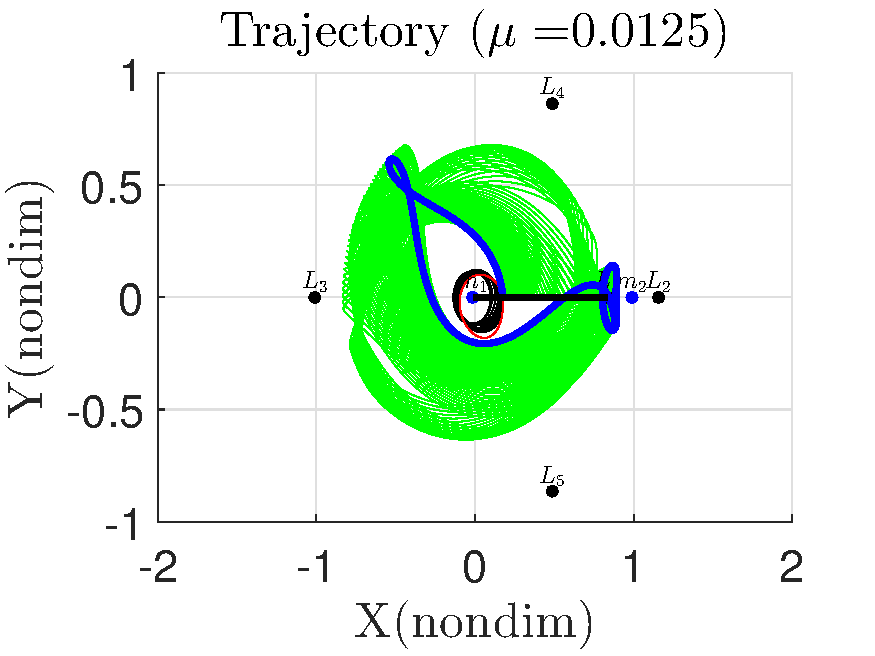
\includegraphics[width=\textwidth]{geo_transfer_full} 
		\caption{Transfer trajectory} \label{fig:gull} 
	\end{subfigure}~ %add desired spacing between images, e. g. ~, \quad, \qquad, \hfill etc. %(or a blank line to force the subfigure onto a new line) 
	\begin{subfigure}[htbp]{0.5\textwidth} 
		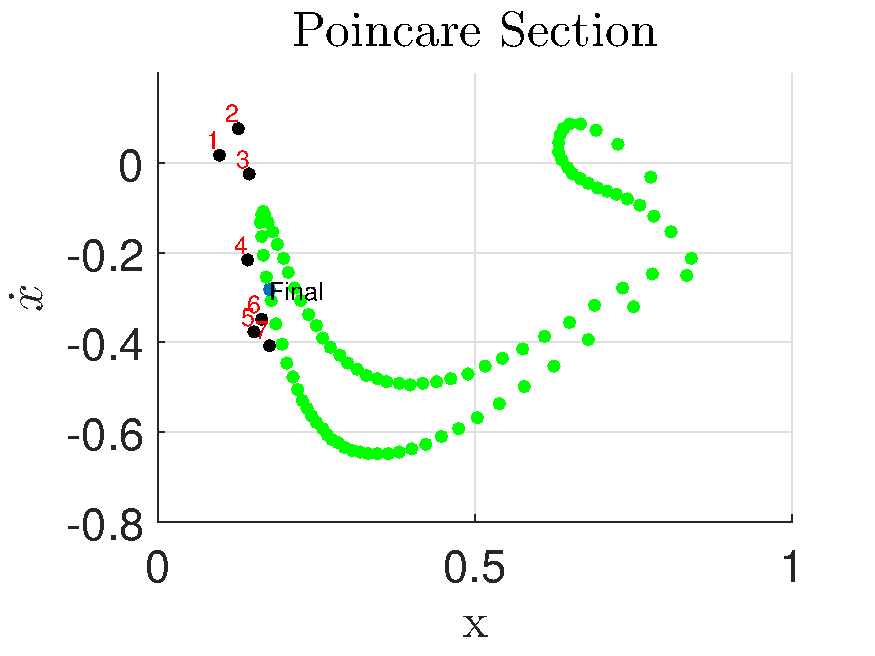
\includegraphics[width=\textwidth]{poincare} 
		\caption{Maximum states on reachability set} \label{fig:tiger} 
	\end{subfigure} 
	\caption{Geostationary to \(L_1 \) transfer in Earth-Moon system}
	\label{fig:geo_transfer} 
\end{figure}



\bibliographystyle{AAS_publication}   % Number the references.
%\bibliography{references}   % Use references.bib to resolve the labels.
\bibliography{library}

\end{document}
